%%% LaTeX Template: Curriculum Vitae
%%%
%%% Source: http://www.howtotex.com/
%%% Feel free to distribute this template, but please keep the referal to HowToTeX.com.
%%% Date: July 2011

%%% ------------------------------------------------------------
%%% BEGIN PREAMBLE
%%% ------------------------------------------------------------
\documentclass[paper=a4,fontsize=11pt]{scrartcl}                % KOMA-article class

%\usepackage[english]{babel}                                % English language/hyphenation
%\usepackage[protrusion=true,expansion=true]{microtype}     % Better typography
\usepackage{amsmath,amsfonts,amsthm}                    % Math packages
\usepackage[pdftex]{graphicx}                               % Enable pdflatex
\usepackage[svgnames]{xcolor}                           % Colors by their 'svgnames'
\usepackage{geometry}
    \textheight=700px                                   % Saving trees ;-) 
\usepackage{url}                                        % Clickable URL's
\usepackage{wrapfig}                                    % Wrap text along figures

\frenchspacing                                  % Better looking spacings after periods
\pagestyle{empty}                               % No pagenumbers/headers/footers
%\usepackage{bbding}                                    % Symbols

%%% Custom sectioning (sectsty package)
%%% ------------------------------------------------------------
\usepackage{sectsty}                            % Custom sectioning (see below)

\sectionfont{%                                  % Change font of \section command
    \usefont{OT1}{phv}{b}{n}%                   % bch-b-n: CharterBT-Bold font
    \sectionrule{0pt}{0pt}{-5pt}{3pt}
    }

%%% Macros
%%% ------------------------------------------------------------
\newlength{\spacebox}
\settowidth{\spacebox}{8888888888}              % Box to align text
\newcommand{\sepspace}{\vspace*{1em}}           % Vertical space macro

\newcommand{\MyName}[1]{
        \Huge \usefont{OT1}{phv}{b}{n} \hfill #1        % Name
        \par \normalsize \normalfont}

\newcommand{\MySlogan}[1]{
        \large \usefont{OT1}{phv}{m}{n}\hfill \textit{#1} % Slogan (optional)
        \par \normalsize \normalfont}

\newcommand{\NewPart}[1]{\section*{\uppercase{#1}}}

\newcommand{\PersonalEntry}[2]{
        \noindent\hangindent=2em\hangafter=0        % Indentation
        \parbox{\spacebox}{                     % Box to align text
        \textit{#1}}                                % Entry name (birth, address, etc.)
        \hspace{1.5em} #2 \par}                 % Entry value

\newcommand{\SkillsEntry}[2]{                       % Same as \PersonalEntry
        \noindent\hangindent=2em\hangafter=0        % Indentation
        \parbox{\spacebox}{                     % Box to align text
        \textit{#1}}                                % Entry name (birth, address, etc.)
        \hspace{1.5em} #2 \par}                 % Entry value   

\newcommand{\EducationEntry}[4]{
        \noindent \textbf{#1} \hfill                    % Study
        \colorbox{Black}{%
            \parbox{10em}{%
            \hfill\color{White}#2}} \par                % Duration
        \noindent \textit{#3} \par                  % School
        \noindent\hangindent=2em\hangafter=0 \small #4  % Description
        \normalsize \par}

\newcommand{\WorkEntry}[4]{                     % Same as \EducationEntry
        \noindent \textbf{#1} \hfill                    % Jobname
        \colorbox{Black}{%
            \parbox{10em}{%
            \hfill\color{White}#2}} \par        % Duration
        \noindent \textit{#3} \par                  % Company
        \noindent\hangindent=2em\hangafter=0 \small #4  % Description
        \normalsize \par}



%%% ------------------------------------------------------------
%%% BEGIN DOCUMENT
%%% ------------------------------------------------------------
\begin{document}
\begin{wrapfigure}{l}{0.5\textwidth}
    \vspace*{-2em}
        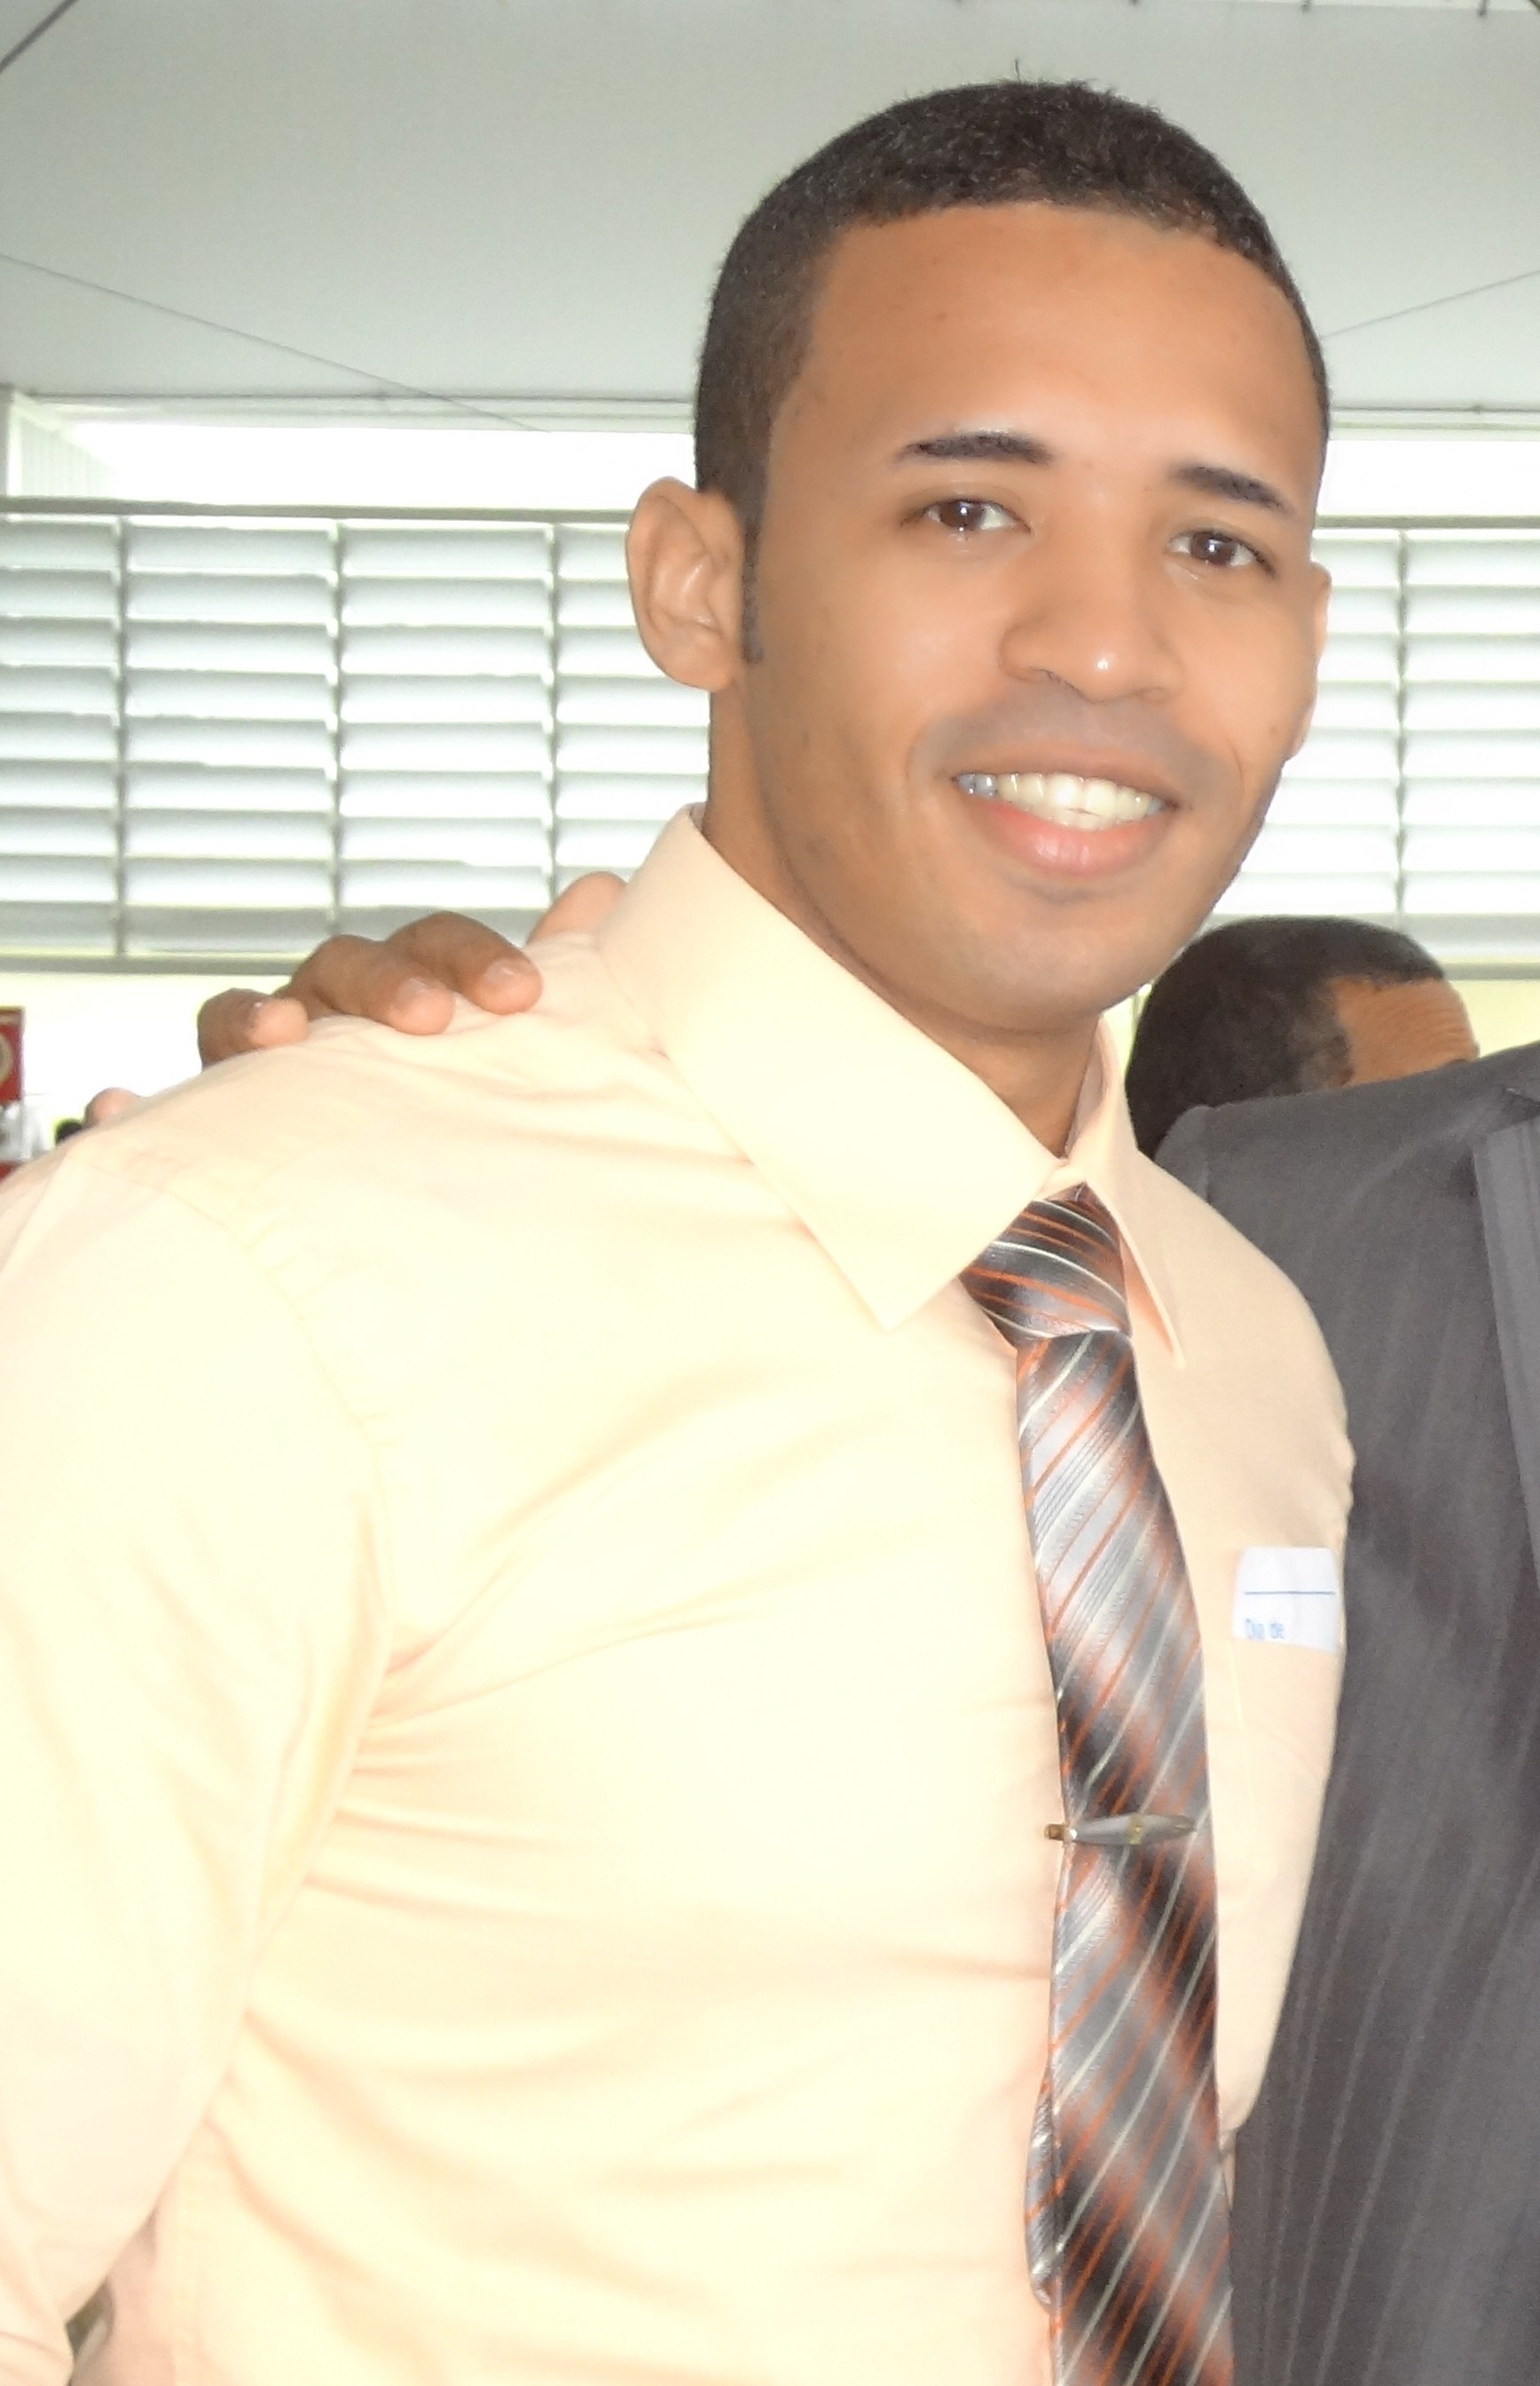
\includegraphics[width=0.15\textwidth]{patrono}
\end{wrapfigure}
\MyName{Rodrigo de Santana Santos}
\MySlogan{Curriculum Vitae}

\sepspace

%%% Personal details
%%% ------------------------------------------------------------
\NewPart{Informa\c c\~oes Pessoais}{}

\PersonalEntry{Nascimento}{Junho 28, 1986} 
\PersonalEntry{Endere\c co}{Rua da Mangueira 60, Pero Vaz, Salvador - BA	}
\PersonalEntry{Telefones}{(71) 82495732 (claro) / 88281568 (oi)  }
\PersonalEntry{e-mail}{\url{rodrigo_geofisico@hotmail.com}}

%%% Education
%%% ------------------------------------------------------------
\NewPart{Forma\c c\~ao}{} 

\EducationEntry{Mestrando em Geof\'isica}{Atual}{Universidade Federal da Bahia - UFBA}{Em andamento.}
\sepspace

\EducationEntry{Bacharelado em Geof\'isica}{2012-2014}{Universidade Federal da Bahia - UFBA}{O curso de Geof\'isica da UFBA tem direcionamento para o uso da s\'ismica na explora\c c\~ao de hidrocarbonetos. Para tal os alunos s\~ao submetidos ao aprendizado de das ci\^encias F\'isica, Matem\'atica e Geologia com uso de linguagens computacionais avan\c cadas.}
\sepspace

\EducationEntry{Bacharelado em F\'isica {\it (parcial)}}{2010-2012}{Universidade Federal da Bahia - UFBA}{Curso de F\'isica da UFBA \'e um curso de ci\^encias. Curso no qual frequentei regularmente durante os quatro primeiro semetre (2010-2012), at\'e o momento em que o tranquei.}

%%% Work experience
%%% ------------------------------------------------------------
\NewPart{Experi\^encias Profissionais}{}
\EducationEntry{Monitor de F\'isica - PIBID}{2011}{Universidade Federal da Bahia - UFBA}{Atuante como monitor de F\' isica do projeto PIBID em turmas do primeiro ao terceiro ano do n\'ivel  m\'edio nos col\'egios Thales de Azevedo e Col\'egio Estadual da Bahia.}
\sepspace
\EducationEntry{Professor de F\'isica}{2011-2012}{Pr\'e-vestibular ONG Oficina de Cidadania}{Atuante como professor de F\'isica do cursinho preparat\'orio para o vestibular.}
\sepspace
\EducationEntry{Professor de F\'isica}{2012}{Colegio Estadual da Bahia}{Atuante como professor estagi\'ario em turmas do primeiro ao terceiro ano do n\'ivel  m\'edio.}
\sepspace
\EducationEntry{Professor de Matem\'atica}{2012-2013}{Pr\'e-vestibular ONG Oficina de Cidadania}{Atuante como professor de Matem\'atica.}
\sepspace
\EducationEntry{Professor de F\'isica}{2014 - 2015}{Pr\'e-vestibular Universidade Para Todos}{Atuante como professor de F\'isica do cursinho preparat\'orio para o vestibular. }%Eleito em 2014, pelos alunos, o melhor professor dos quatro polos onde foi atuante.}
\vspace{.5cm}
\sepspace

\EducationEntry{Professor Monitor de F\'isica}{2014.1-2014.2}{Universidade Federal da Bahia - UFBA}{Atuante como professor monitor da disciplina F\'isica geral e experimental II-E na UFBA durante o ano de 2014.}
\sepspace
\EducationEntry{Professor de Matem\'atica}{2014 - 2015}{Pr\'e-vestibular Universidade Para Todos}{Atuante como professor de Matem\'atica do cursinho preparat\'orio para o vestibular.}% Dono de cinco turmas, as quais o elegeu como o melhor e mais paciente professor de matemática.}


%%% Skills
%%% ------------------------------------------------------------
\NewPart{Habilidades}{}

\SkillsEntry{Idiomas}{Portugu\^ es (L\'inguas Maternas)}
\SkillsEntry{}{Ingl\^es (Intermedi\'ario)}
%\SkillsEntry{}{German (fluent)} 

\SkillsEntry{Software}{\textsc{Sismic Unix}, \textsc{Gnuplot},  \LaTeX, Fortran90 e C }


%%% References
%%% ------------------------------------------------------------
\NewPart{Produ\c c\~ao Cient\'ifica}{}
\EducationEntry{Apresenta\c c\~ao em Poster}{2014}{Reuni\~ao Anual da ANP}{Estudo Avaliativo da  Modelagem Num\'erica de Tempos de Tr\^ansito atrav\'es do Tra\c camento de Raios S\'ismicos - Intrus\~ao Gran\'itica .}
\sepspace
\EducationEntry{Artigo}{2014}{VI Simp\'osio Brasileiro de Geof\'isica}{Estudo Avaliativo da  Modelagem Num\'erica de Tempos de Tr\^ansito atrav\'es do Tra\c camento de Raios S\'ismicos - Camadas Inclinadas.}
\EducationEntry{Artigo}{2015}{VI Congresso Internacional de  Geof\'isica}{Seismic modeling of traveltimes with  rays parameterized by time and arc lenght.}
\sepspace
\end{document}
